\chapter{Evaluation}
\label{c:evalu}

This chapter discuss the end-to-end evaluation of our system.

\section{Evaluation dataset}
\label{s:eval}
For collecting the ground truth data we walked along the path of 300 feet at an urban street to record the video with samrtphone.
We record data at different time of the day and at different light condition.
\ref{f:dataset} shows the scene variation of recored video.
The right one is cloudy and the left one is sunny.

\begin{figure}[!ht]
\centering
\subfloat[Sunny] {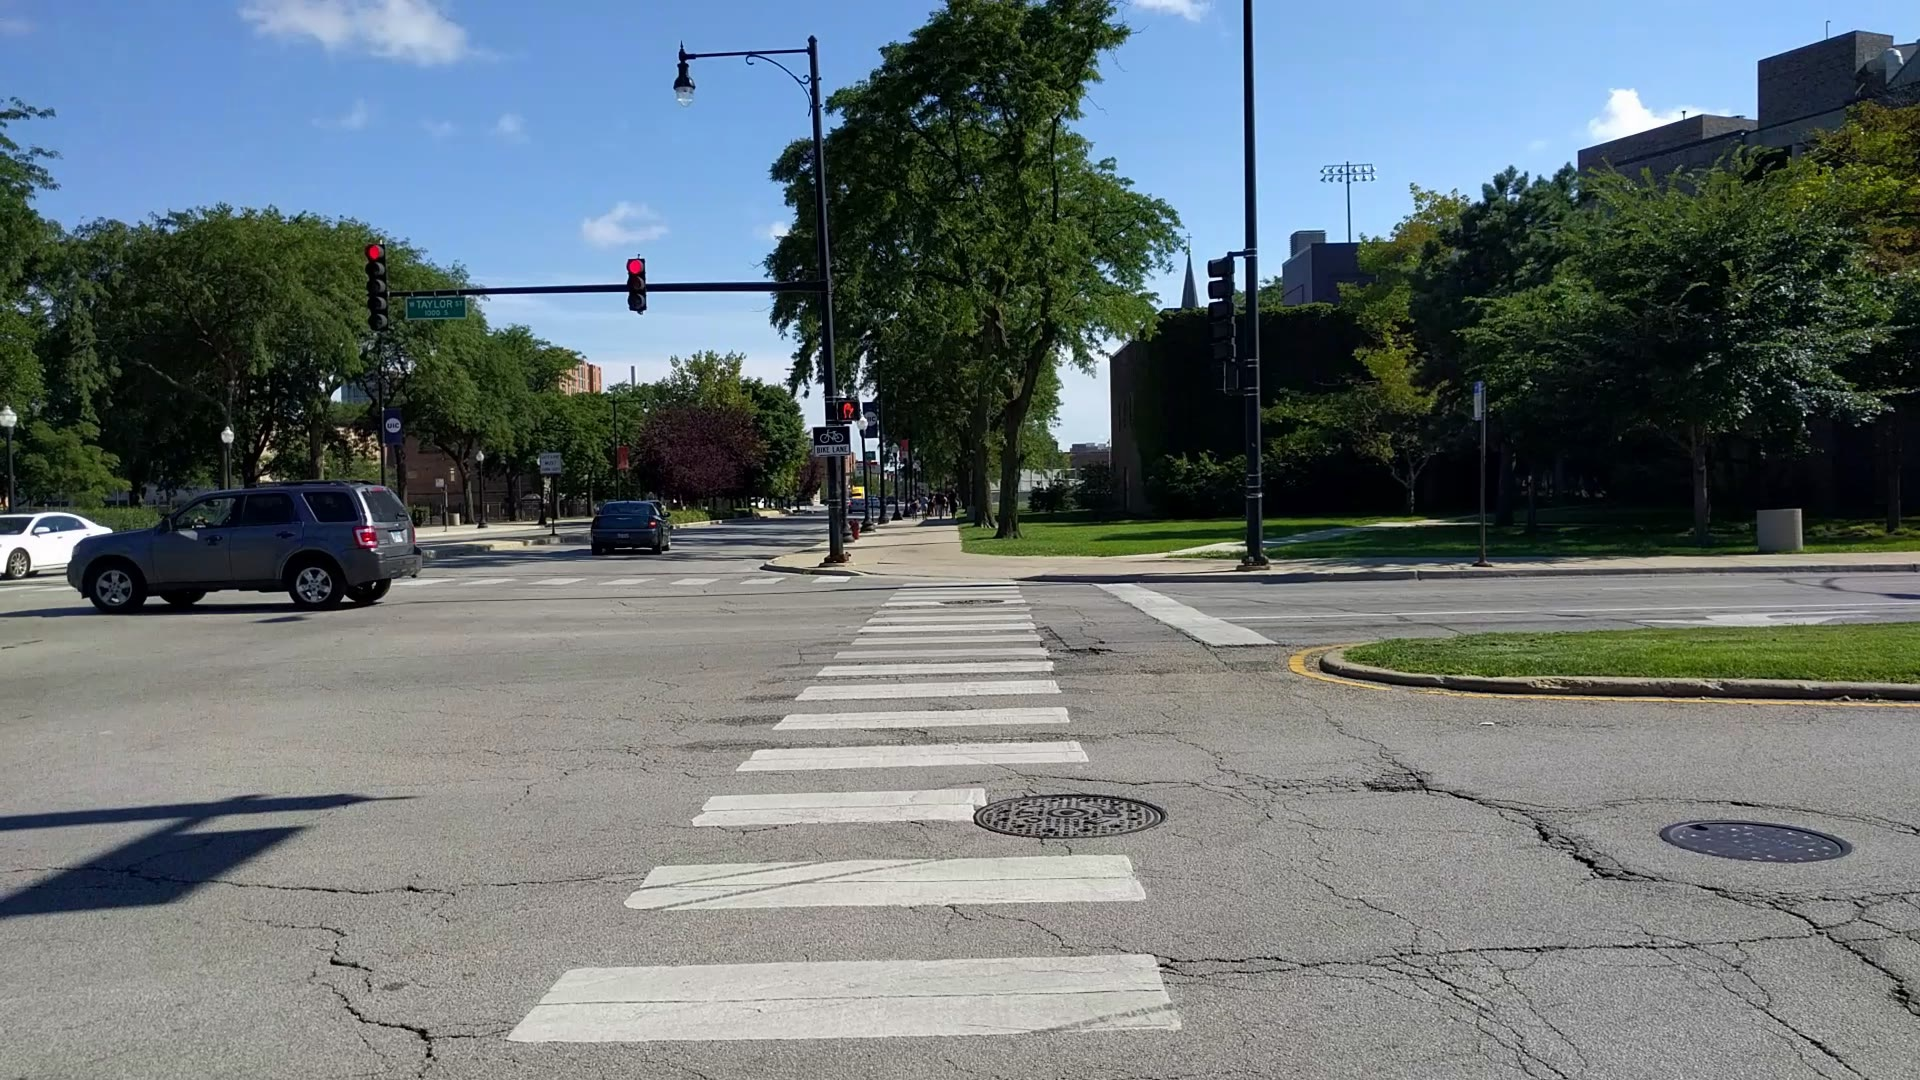
\includegraphics[width=3.1in]{images/sunny.jpg}}
\hfill
\subfloat[Cloudy] {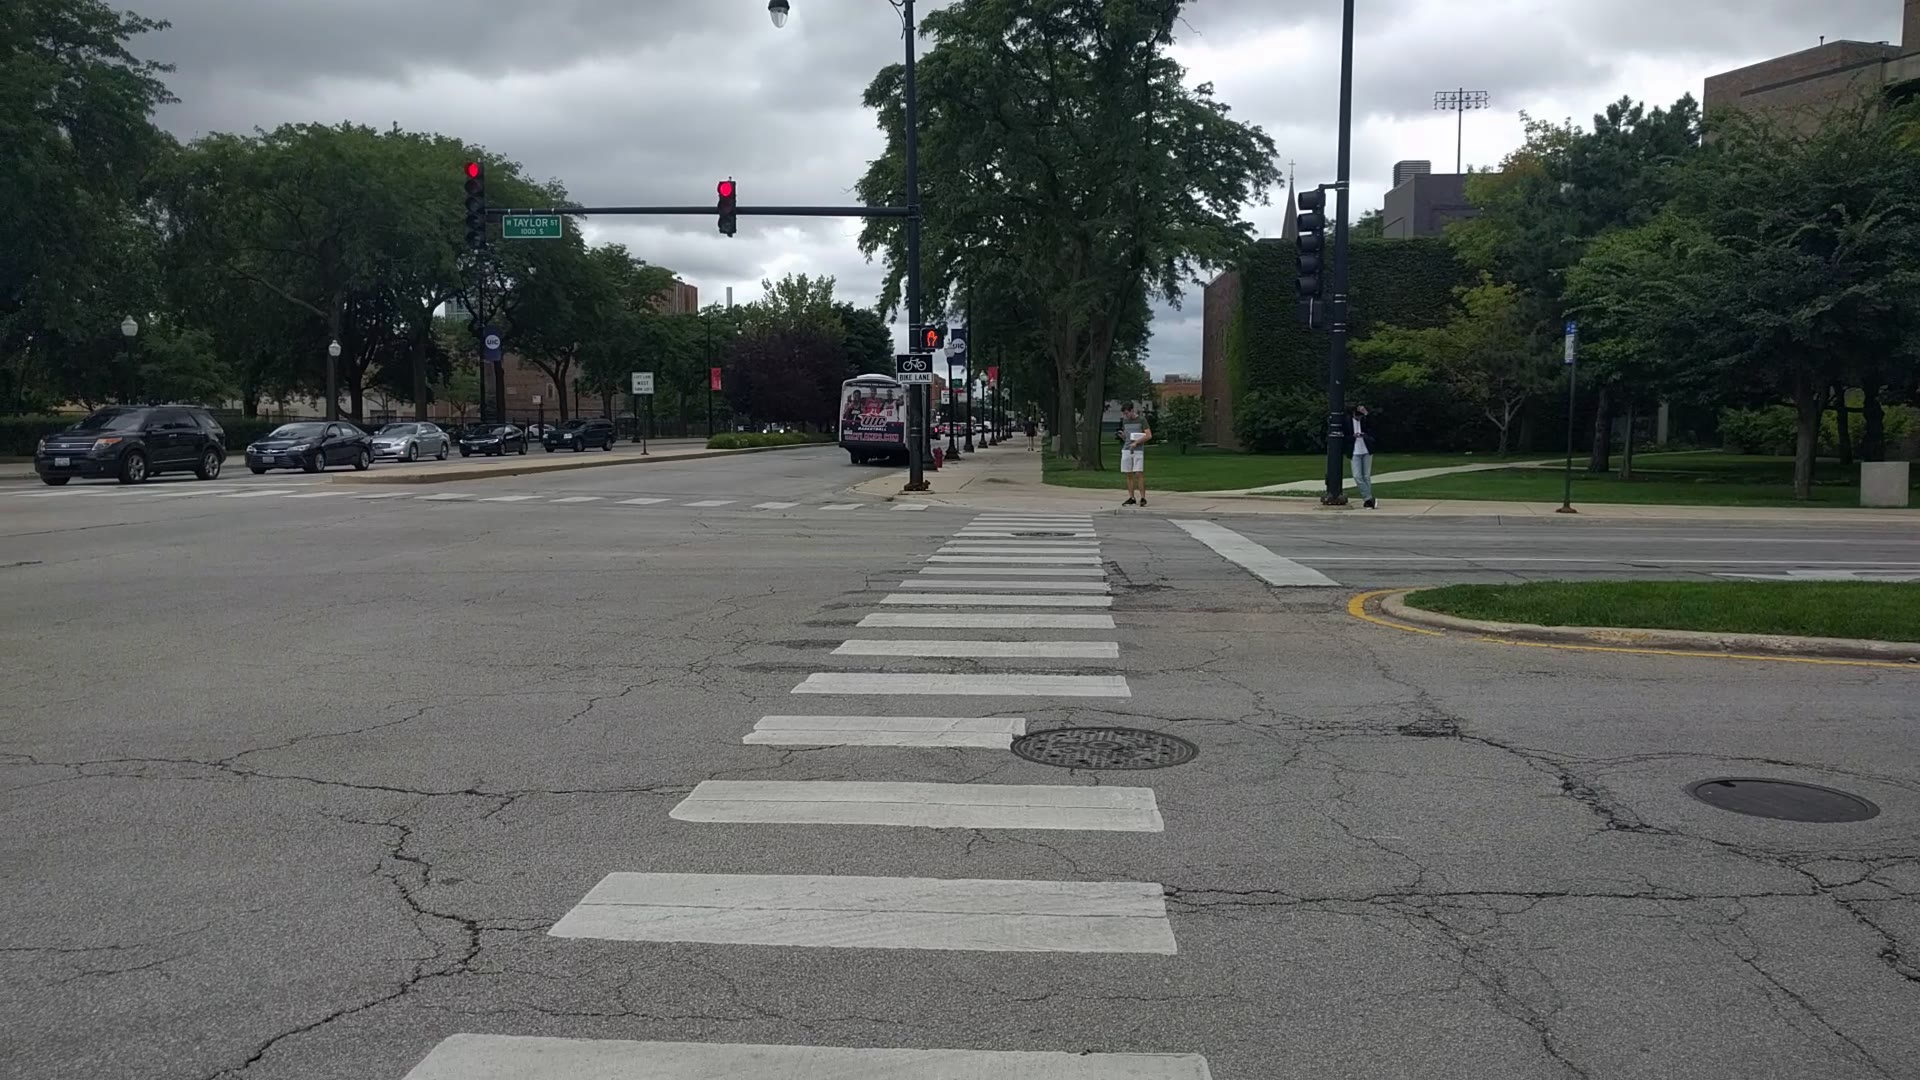
\includegraphics[width=3.1in]{images/cloudy.jpg}}
\caption{Scene variation of recorded video.}
\label{f:dataset}
\end{figure}

\ref{t:dataset} shows the total no of frames, and time duration of our dataset.

\begin{table}[h!]
  \centering
  \caption{Description of the dataset.}
  \label{t:dataset}
  \begin{tabular}{  l  c  r  }
   
    Name & Frame Count & Time Duration \\
    \hline
    Walk with sensor movement-Sunny day & 5905 & 3 mins 16 secs  \\
    Walk with sensor movement-Cloudy day & 6205 & 3 mins 26 secs \\
    Walk regular movement & 6022 & 3 mins 20 secs \\
    Static with sensor movement & 1810 & 1 min \\
    \hline
  \end{tabular}
\end{table}

\section{Annotation}
TODO

\section{Computation time}
We collected data at different time of the day as we discussed in \ref{s:eval}.
In this section we will discuss the processing time of these datasets with the sensor hint and without it.

\begin{figure}[h!]
\centering
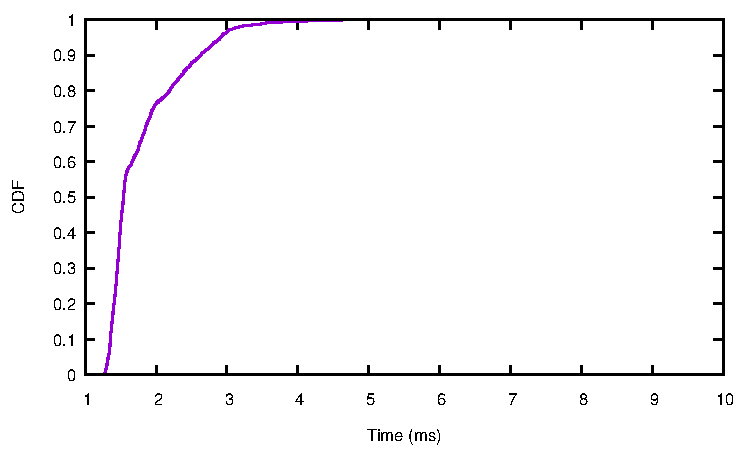
\includegraphics[width=5.2in]{plots/sunny_cdf_filter.pdf}
\caption{CDF of processing time for heuristic filter.}
\label{f:cdf_fil}
\end{figure}

\ref{f:cdf_fil} shows the processing time for the heuristic filter we discuss at \ref{c:sys}.
The processing time depends on the number of circle detected on the frame.
If circle count is high, filtering need for all of these circles, so processing time will be higher.
\ref{f:cdf_fil} shows that the median processing time is 1.5 secs for the filtering. 

\begin{figure}[h!]
\centering
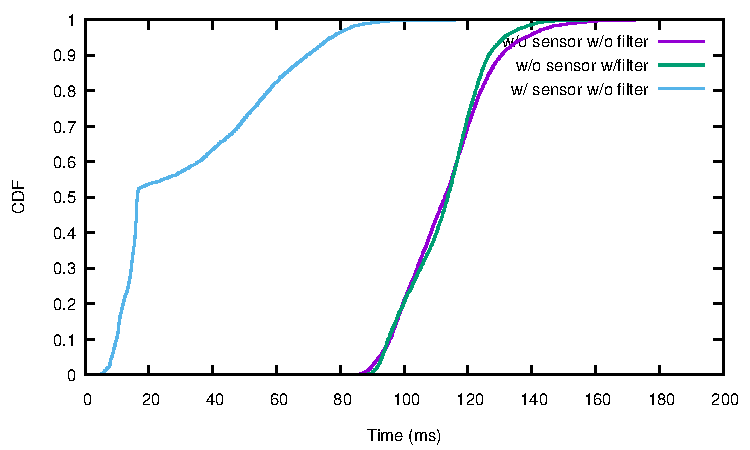
\includegraphics[width=5.2in]{plots/sunny_cdf_time.pdf}
\caption{CDF of frame processing time for walking dataset in sunny weather.}
\label{f:cdf_sunny}
\end{figure}

\begin{figure}[h!]
\centering
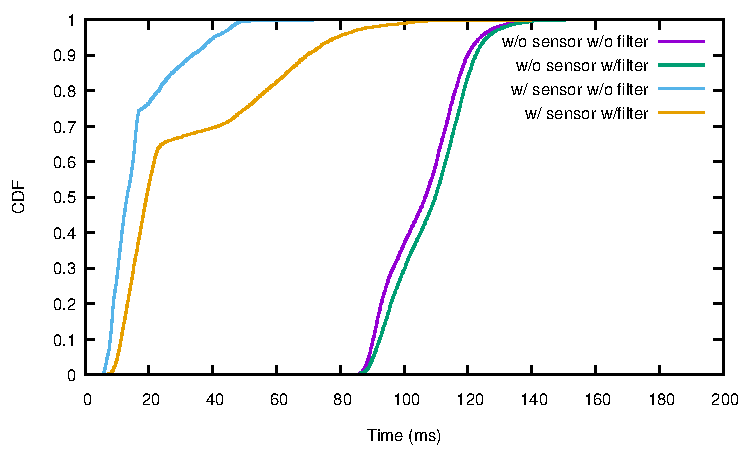
\includegraphics[width=5.2in]{plots/walk_cdf_time.pdf}
\caption{CDF of frame processing time.}
\label{f:cdf_time}
\end{figure}

\ref{f:cdf_time} shows the CDF of the processing time.
It shows that the median of the processing time without sensor and any heuristic filter is 106ms.
Wheather, the median of the processing time with sensor and without heuristic filter is 13ms.
We can improve the processing time 8.15x.
The median of the processing time witt sensor and heuristic filter is 19ms.
Though we can improve the processing time 5.57x with the filter but it increases the accuracy, which we will describe at section \ref{s:acc}

\begin{figure}[h!]
\centering
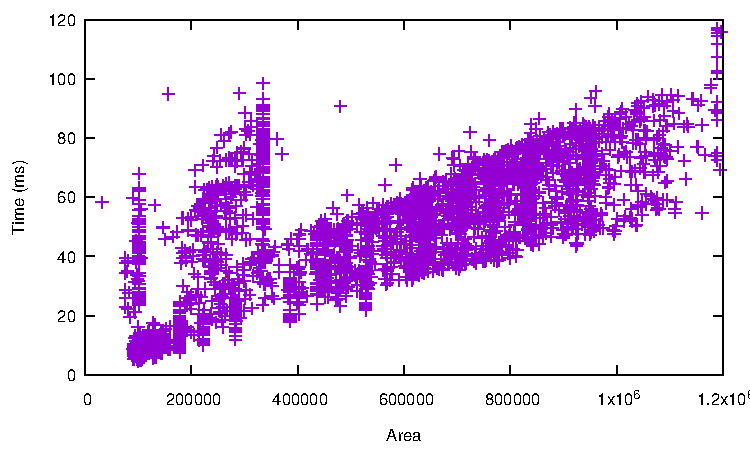
\includegraphics[width=5.2in]{plots/sunny_recarea.pdf}
\caption{Processing time with the increase of the rectangle area.}
\label{f:recarea}
\end{figure}


\section{Accuracy}
\label{s:acc}
To demonstrate the robustness of the various traffic light scenarios, we recorded video at different lightening condition: cloudy and sunny and at different time of the day.
We walked along the intersection of the street and the route consist of 16 traffic light.

\ref{t:con_nocrp} shows a confusion matrix for the traffic light decision when we do not consider the sensor hints of the smartphone.
\ref{t:con_crp} shows the confusion matrix considering the sensor hints in the same dataset.

\begin{table}[h!]
  \centering
  \caption{Confusion Matrix without sensor hints for static movement dataset.}
  \label{t:con_nocrp}
  \begin{tabular}{  l | c | c | r }
   
     & Detected Red & Detected Green &  \\
    \hline
    Actual Red & 828 & 1 & 99.88\% \\
    \hline
    Actual Green & 54 & 509 & 90.41\% \\
    \hline
    & 93.88\% & 98.8\% & 96.05\% \\
    
  \end{tabular}
\end{table}

\begin{table}[h!]
  \centering
  \caption{Confusion Matrix with sensor hints for static movement dataset.}
  \label{t:con_crp}
  \begin{tabular}{  l | c | c | r }
   
     & Detected Red & Detected Green &  \\
    \hline
    Actual Red & 909 & 1 & 99.89\% \\
    \hline
    Actual Green & 36 & 524 & 93.57\% \\
    \hline
    & 96.19\% & 99.81\% & 97.48\% \\
    
  \end{tabular}
\end{table}

These results show that, using the sensor hints our system is more accurate detecting the red light and also false detection of green light is decreasing.

\ref{f:tp_stat} shows the detection rate for the red and green state of the traffic light.
It shows that using the sensor hints detection rate for red light increases from 86\% to 96\% and for green light, detection rate increases 96\% to 99\%.

\begin{figure}[h!]
\centering
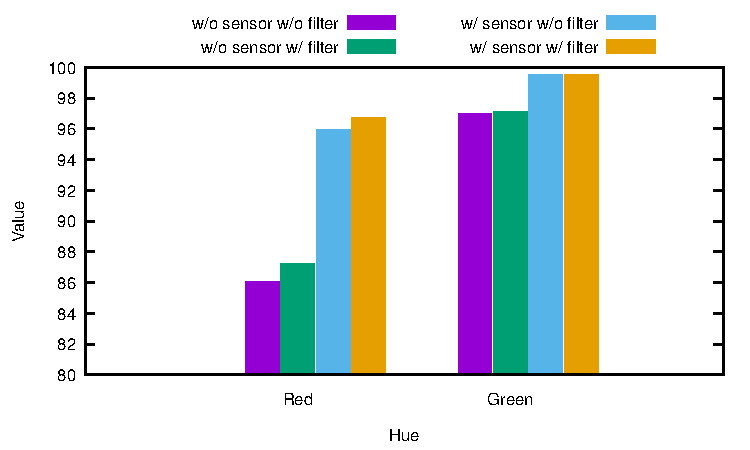
\includegraphics[width=5.2in]{plots/bar_tp.pdf}
\caption{Detection rate for static movement dataset.}
\label{f:tp_stat}
\end{figure}

\ref{f:fp_stat} shows the misdetection rate for the red and green state of traffic light.
Left one is the false positive detection and the right one is the false negative detection for the traffic light detection.

\begin{figure}[!ht]
\centering
\subfloat[] {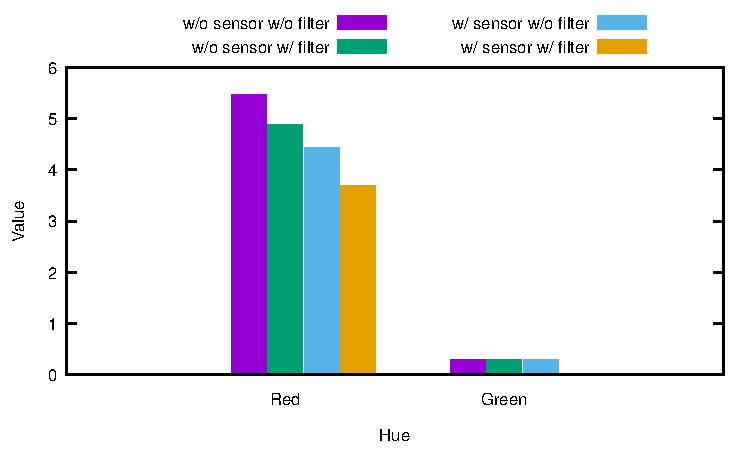
\includegraphics[width=3.1in]{plots/bar_fp.pdf}}
\hfill
\subfloat[] {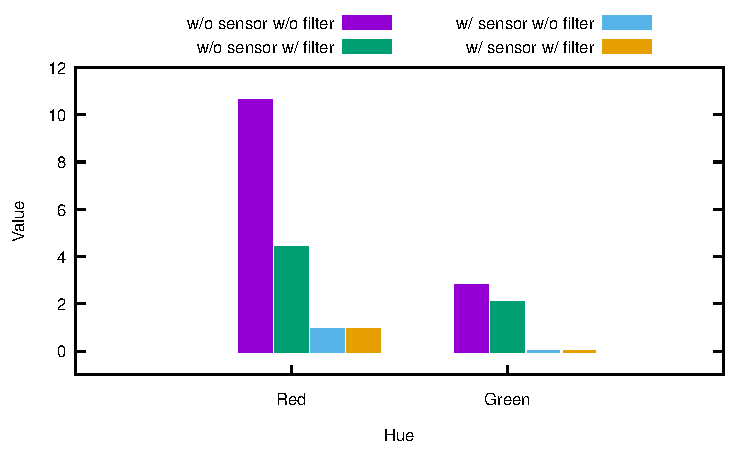
\includegraphics[width=3.1in]{plots/bar_fn.pdf}}
\caption{Misdetection rate for static movement dataset.}
\label{f:fp_stat}
\end{figure}

\ref{t:acc_stat} shows the accuracy rate for the static movement dataset.
It shows that the accuracy increases from 89\% to 97\%.

\begin{table}[h!]
  \centering
  \caption{Accuracy for detection.}
  \label{t:acc_stat}
  \begin{tabular}{  l  c | r  }
   
     & without sensor & with sensor  \\
    \hline
    & 89.7313\% & 97.035\%  \\
    \hline
  \end{tabular}
\end{table}





